\chapter{Context and Objectives}
\pagenumbering{arabic}
\section{Aim and Outline of the master thesis}
The Boston Dynamic's Spot robot equipped with a LiDAR sensor provides perspectives of autonomous navigation through the utilization of a pre-implemented service known as GraphNav, or, by implementing a SLAM algorithm as previously explored in Achille's master thesis \cite{AchilleThesis}.\\
Autonomous navigation enables novel applications, including tracking construction sites using the robot, by recording and mapping a point cloud of its surrounding environment.\\

A significant application of the recorded point cloud is its comparison with other point clouds and detect their differences. Those other point clouds can originate from previous records, or, from a theoretical model known as a building information model (BIM). The objective is to identify changes or faults that may occur during construction.\\

This master thesis investigates 2 different approaches to detecting those changes, specifically, focusing on translation and rotation changes. The first approach employs different computer vision techniques which allow the detection, classification, and segmentation of these changes. The second one is based on a deep learning approach, drawing inspiration from recent progress in point cloud classification and semantic segmentation.\\

More precisely, to enable the evaluation and comparison of both approaches, a dataset representing walls and buildings was generated. The performance of each approach is assessed using different metrics for classification and semantic segmentation tasks. And conclusions about the deep learning approach are drawn, in comparison to the classical method, showing some perspective for future application.\\

Chapter 1 provides an overview of the context and technologies employed, including the Spot robot provided by Buildwise and the LiDAR sensor utilized for capturing point cloud data.\\ 

Afterward, the first approach referred as the classical approach, is described from Chapter 2 to Chapter 4. Each chapter details a step within the deterministic method, including point cloud registration, plane detection, plane matching, and change detection.\\

Chapter 5 introduces the second approach. Relevant definitions and models are described alongside the presentation of our proposed network architecture.\\

Finally, Chapter 6 delves into the implementation details and provides a comprehensive analysis of the results obtained from the evaluation of these two approaches across various metrics.

\section{Point Cloud}
In a wide range of applications like robotics, architecture, virtual reality, and many more, it is important to detail information about the surrounding environment. Specifically, in the context of change detection and monitoring construction sites, there is a need to accurately depict buildings and objects using a 3D model.\\

To achieve this, point clouds are commonly employed. Point clouds represent a set of unordered discrete data points, where each point lies on a frame described by its cartesian coordinates. Typically, these points mainly represent surfaces providing a description of objects and environment.\\

Point clouds can be generated through various techniques including Light Detection and Ranging (LiDAR) sensors which use laser beams to capture spatial information, RGB-D cameras which exploit the depth to reconstruct the surrounding, or structure-from-motion (SFM) which leverage multiple images taken from different angles \cite{pcdAcquisition}.

\begin{figure}[ht]
    \begin{subfigure}{.48\linewidth}
    \centering
    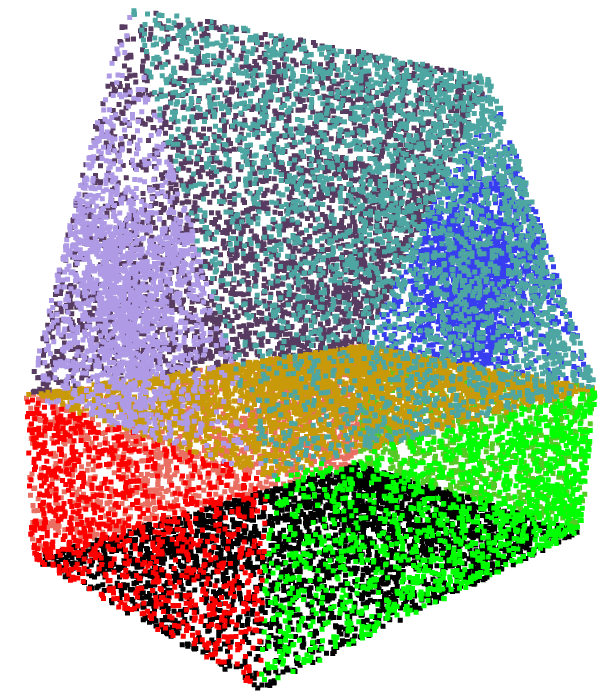
\includegraphics[scale=0.4]{Img/00_Maison.png}
    \end{subfigure}
    \begin{subfigure}{0.48\linewidth}
    \centering
    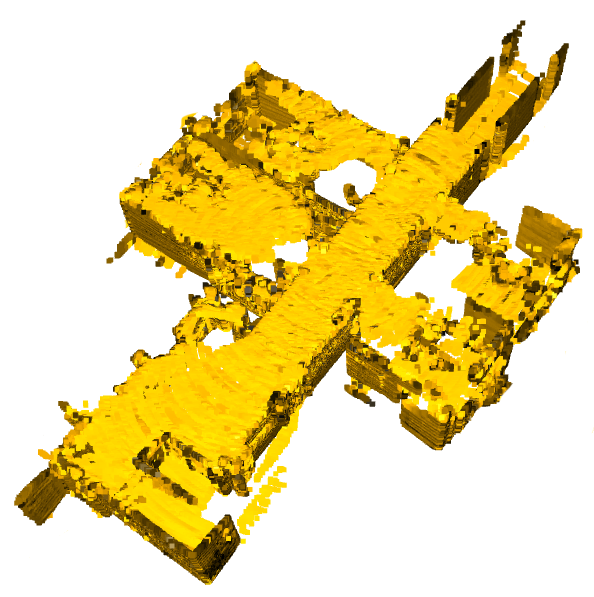
\includegraphics[scale=0.5]{Img/00_cstc.png}
    \end{subfigure}\\
\caption{Two examples of point clouds: A house with colored surfaces for visualization and a Buildwise's floor containing a hallway and four connected rooms.}
\end{figure}


\section{SPOT}
Spot is an agile mobile robot capable to navigate in various environments such as construction sites and rough terrains. Moreover, with the help of the Spot SDK, developers and operators can make Spot do repetitive tasks and automate routine inspections \cite{Spot}.\\

The robot itself possesses 12 degrees of freedom, with 3 degrees per leg. It has the capability to carry a payload weighing up to $14$ kg. The estimated autonomy is around 90 minutes for run time and $180$ minutes for standby time. Furthermore, it is designed to operate within a temperature range spanning from $-20^{\circ}$C to $45^{\circ}$C \cite{Spotcharact}.
\begin{figure}[ht]
    \begin{subfigure}{.48\linewidth}
    \centering
    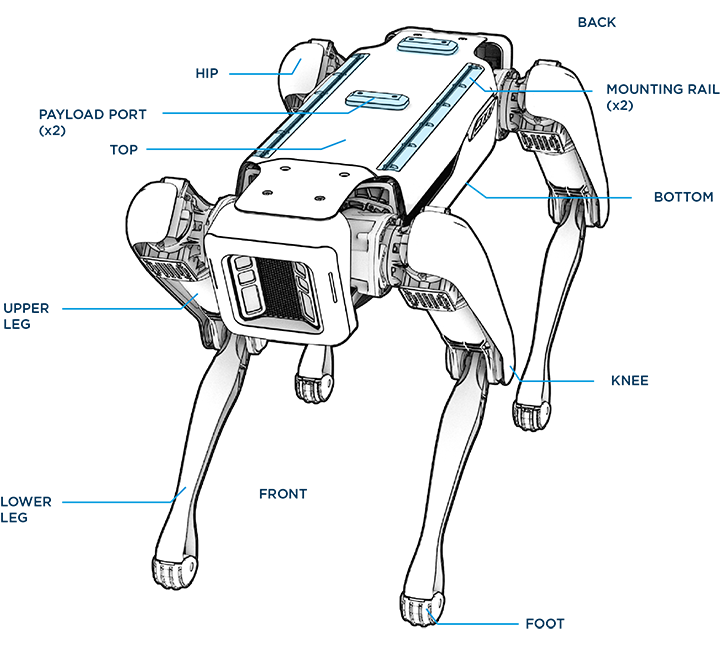
\includegraphics{Img/00_SPOT3.png}
    \end{subfigure}
    \begin{subfigure}{0.48\linewidth}
    \centering
    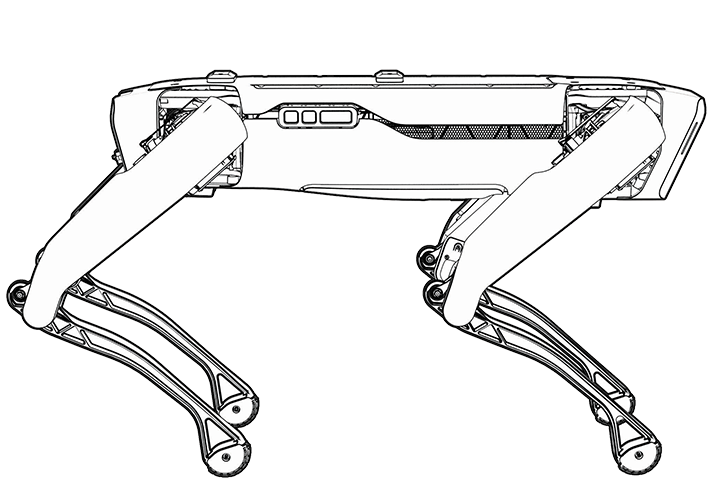
\includegraphics[scale=0.3]{Img/00_SPOT1.png}
    \end{subfigure}\\
\caption{Front and side views of Spot with its main physical features \cite{Spotcharact}.}
\end{figure}

\subsection{Geometry and Frames}
Spot use frames in order to help him navigate in the world. While moving, Spot keeps track of frames such as its body frame, its sensor frames, the inertial frame, objects frames (detected object in its surrounding) and many more \cite{SpotFrames}. \\

In order to keep a coherent world, Spot applies spatial transformations to monitor relationships between those different frames. The transformation between two frames is defined by a translation vector $[x,y,z]$ which indicates the difference between both origin and a rotation quaternion $[w,x,y,z]$ which indicates the difference between the axis orientations \cite{quaternion}.\\


Those rigid transformations between frames can also be expressed with a single transformation matrix with homogeneous coordinates. The shape of the transformation matrix is given as follows:
\begin{equation}
    T = 
    \begin{pmatrix}
        \textbf{R} & \textbf{t}\\
        \textbf{0} & 1
    \end{pmatrix}
\end{equation}
where $\textbf{R} \in \mathbb{R}^{3 \times 3}$ is the rotation matrix, $\textbf{t} \in \mathbb{R}^3$ is the translation matrix while $1$ is a scalar.\\

More explicitly, if $T_{A\rightarrow B}$ is the transformation matrix between frame $A$ and frame $B$, for a given point in frame A $(x_A, y_A, z_A)$, this point's coordinate in frame $B$ can be found using $T_{A\rightarrow B}$.
\begin{equation}\label{eq:TransfoMatrix}
    \begin{pmatrix}
        x_B \\ y_B \\ z_B
    \end{pmatrix}
    =
    \underbrace{
    \begin{pmatrix}
        \textbf{R} & \textbf{t}\\
        \textbf{0} & 1
    \end{pmatrix}}_\text{$:= T_{A\rightarrow B}$}
    \begin{pmatrix}
        x_A \\ y_A \\ z_A
    \end{pmatrix}
\end{equation}

\subsection{Autonomy Services}
Spot robot features a mapping, localization, and autonomous navigation system, known as GraphNav, which consists of on the one hand a service used on the robot and on the other hand an API for the development of autonomous navigation behavior \cite{SpotAutonomy}.\\ 

In order to make Spot do an automated routine, a map recording must be done first. This map, representing the world and generated by GraphNav, consists of edges and waypoints: 

\begin{itemize}
    \item A waypoint represents an area in the world that is accessible for the robot by navigation. During a map recording, it is created approximately every two meters. It consists of a reference frame, a name, a unique ID, annotations, and sensor data. A waypoint contains a snapshot that bundles those data in one unit.

    \item An edge in a map represents how the robot moves and the relationship in 3D space between the two waypoints. It involves relative poses between two waypoints and also information about how the robot should move along that edge.

\end{itemize}

Once the new map is recorded, if an operator wants Spot to make repetitive tasks, the robot must have its localization initialized. As illustrated in Figure \ref{fig:Spot_init}, a way to initialize the robot is to set the localization near a specific fiducial (such as an AprilTag) that is previously recorded.\\

Once the robot's initial localization has been established, it will consistently monitor its position in relation to waypoints present on the recorded map. As the robot moves in the map, the waypoint used for localization transitions to a neighboring waypoint. \\

In the Spot tablet app, a feature called Autowalk is available. This feature is built upon GraphNav and allows the robot operator to record a GraphNav map and do repetitive missions. 
\begin{figure}[ht]
    \centering
    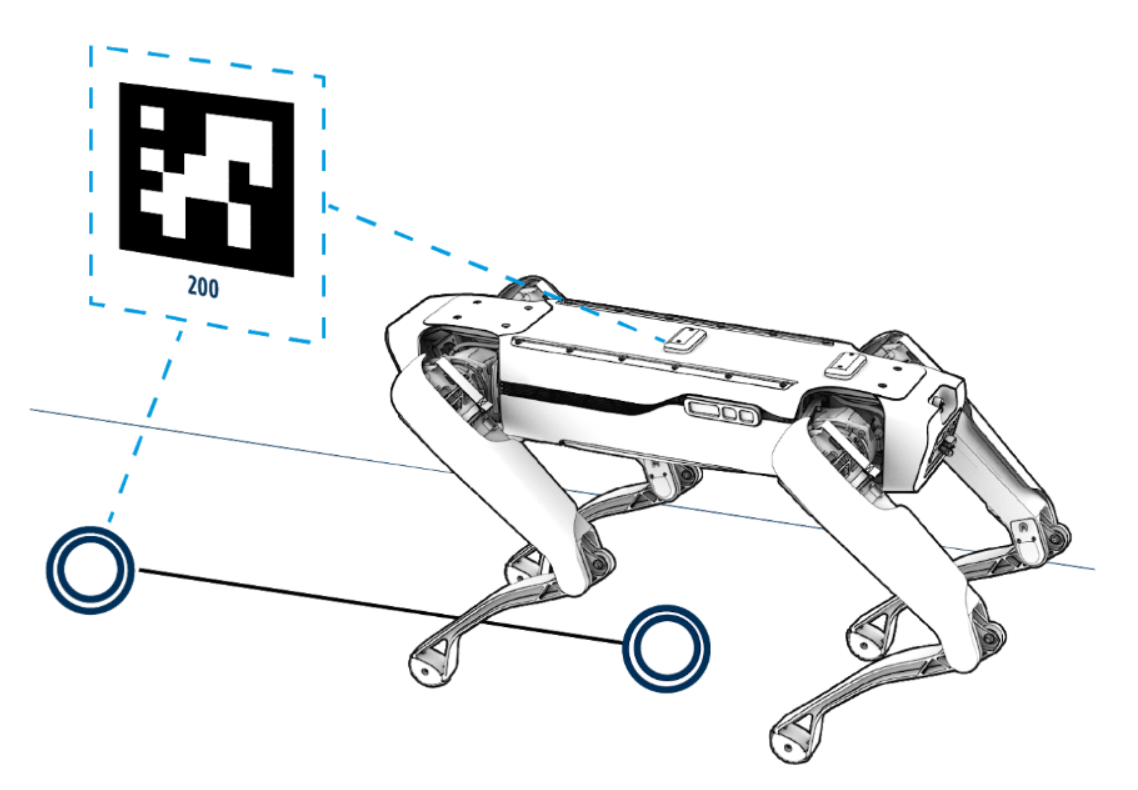
\includegraphics[scale=0.5]{Img/00_SPOT2.png}
    \caption{Illustration of waypoints, edges and Spot initialization with an AprilTag \cite{SpotAutonomy}. }
    \label{fig:Spot_init}
\end{figure}
\section{Simultaneous localization and mapping}
In the case of monitoring construction sites, drastic changes can happen between 2 map records: New walls can be built, and more obstacles appear as the building is constructed. \\

Because of the dynamic nature of the construction site, Spot autonomy services may not be sufficient to offer real autonomy and the robot need to be able to simultaneously locate itself and map the world as the robot is moving. This common problem is also known as Simultaneous Localization and Mapping (SLAM) problem.\\

Common algorithm to solve the SLAM problem belongs either to the filtering approaches or the smoothing approaches \cite{AchilleThesis}.  
\begin{itemize}
    \item Filtering approaches use an on-line description of the SLAM problem. Popular methods such as the Kalman filter, Extended Kalman filter, and Particle filters belong to this category.\\
    More explicitly, the on-line description means that those methods estimate for every discrete time $t$, the \textbf{robot’s pose} $x_t$ and the map $m$ based on its odometry history $u_{1:t}$ and measurement history $z_{1:t}$ derived from LiDAR.

    \item Smoothing approaches use a full description of the SLAM problem. Graph-based optimization such as GraphSLAM belongs to this category.\\
    More explicitly, the full description means that those method estimate for every discrete time $t$, the \textbf{full robot’s trajectory} $x_{1:t}$ and the map $m$ based on its odometry history $u_{1:t}$, measurement history $z_{1:t}$ (derived from LiDAR, cameras,...).\\
\end{itemize}

\section{Light Detection And Ranging}
As previously mentioned, point clouds can be obtained using Light Detection And Ranging (LiDAR) which use laser beams to measure the distance between the source sensor and a targeted object.\\

In order to measure the distance, the LiDAR sensor emits a laser beam in the direction of a target object. This laser beam travels through the air, at a speed similar to the speed of light $c$, and is reflected back to the sensor once it reaches the target. Then, the sensor measures the time $t$ taken for the laser pulse to return and the distance is computed using the equation $d = \frac{c \, t }{2}$.\\

In the specific case of robotic and construction sites, LiDAR sensors can be used for several reasons. Firstly, LiDAR offers good accuracy by exploiting wavelength in the range of 514-1064 nm providing greater spatial resolution than radar and achieving centimeter-level accuracy. Secondly, LiDAR sensors can rapidly capture and process data, delivering real-time information about a robot's surroundings. This is beneficial for tasks such as localization, obstacle detection, path planning and SLAM \cite{AchilleThesis}\cite{LiDAR_review}. \\

\begin{figure}[ht]
    \begin{subfigure}{.48\linewidth}
    \centering
    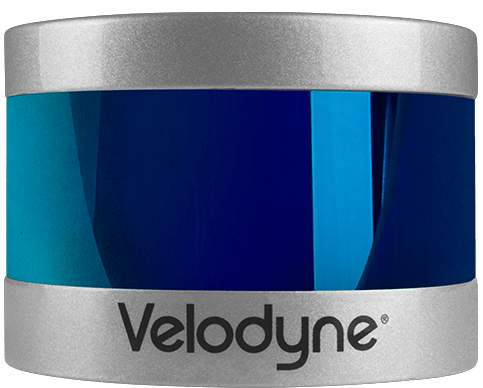
\includegraphics[scale=0.3]{Img/00_VLP-16_1.png}
    \end{subfigure}
    \begin{subfigure}{0.48\linewidth}
    \centering
    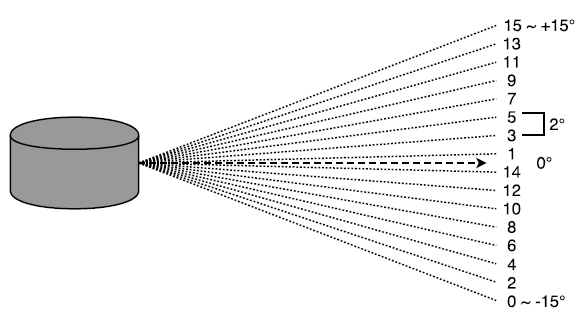
\includegraphics[width = \linewidth]{Img/00_VLP-16_2.png}
    \end{subfigure}\\
\caption{Illustration of Velodyne VLP-16 LiDAR and its vertical range \cite{VLP-photo}\cite{VLP-vertical}.}
\end{figure}

Within the scope of our work, the Velodyne VLP-16 sensor is utilized as the primary sensor. VLP-16 sensor possesses 16 infra-red lasers paired with detectors to measure distances to objects where the vertical field of view obtained is $30 ^{\circ}$ with a vertical resolution of $2 ^{\circ}$. Each laser operates at a firing frequency of $18$ kHz facilitating the acquisition of a set of 3D point data in real-time \cite{VLP-16}.\\

In order to capture a point cloud representing a building, it is necessary to gather distance information in all horizontal directions. With the help of rotating fired lasers with a speed ranging from $5$ Hz to $20$ Hz, VLP-16 achieves a horizontal field of view of $360 ^{\circ}$ \cite{VLP-16}.\\

The obtained point clouds demonstrate a level of accuracy with a measurement noise up to $\pm 3$ cm \cite{LiDAR_review}.





